%! TEX program = xelatex

\documentclass{article}
\usepackage[a4paper, margin=3cm]{geometry}
\setlength{\parindent}{0pt}
\setlength{\parskip}{1em}
\usepackage{fontspec}
\setmainfont{Lato}

\usepackage{amsmath,amssymb,amsthm}
\usepackage{graphicx}
%\usepackage{pgfplots}
%\pgfplotsset{compat=1.16}

\title{}
\author{Mikael Myyrä}
\date{}

\begin{document}

\section*{1.}

Tämä on homogeeninen versio viime kerran tehtävä 3:sta hieman erilaisilla
reunaehdoilla. Nyt mukana on sekä Neumann- että Dirichlet-ehtoja.
Käytetään diskretointia
\[
  \frac{-u_{i,j-1} - u_{i-1,j} + 4u_{i,j} - u_{i+1,j} - u_{i,j+1}}{h^2} = 0.
\]
Keskeisdifferenssikaava Neumann-reunaehdoille on
\[
  \frac{u_{1,j} - 2u_{0,j} + u_{-1,j}}{2h} = 0
\]
alueen vasemmalla reunalla ja
\[
  \frac{u_{i,1} - 2u_{i,0} + u_{i,-1}}{2h} = 0
\]
alareunalla. Tähän tarvitaan haamupisteet $(i,-1)$ ja $(-1,j)$.
Laajentamalla laskenta-alue $([1, N] \times [1, N])$:stä
$([0, N] \times [0, N])$:n saadaan haamupisteiden vaikutus mukaan.

Matlab-koodi:

\begin{verbatim}
% laskenta-alue [0, 1), hilaväli 0.25
STEP_COUNT = 4;
STEP_LENGTH = 1 / STEP_COUNT;

% u:n kerroinmatriisi lohkomatriisina.
% tässä oli viimeksi virhe, jonka takia -1-diagonaalit
% tulivat vääriin kohtiin kun N != 4.
blockT = diag(4*ones(STEP_COUNT, 1)) ...
       - diag(ones(STEP_COUNT - 1, 1), 1) ...
       - diag(ones(STEP_COUNT - 1, 1), -1);
sideDiag = -ones(STEP_COUNT^2 - STEP_COUNT, 1);
uCoefs = blkdiag(repmat({blockT}, 1, STEP_COUNT){:}) ...
       + diag(sideDiag, STEP_COUNT) ...
       + diag(sideDiag, -STEP_COUNT);

% yhtälön oikea puoli on tällä kertaa pelkkiä nollia
% lukuunottamatta yläreunaa y = 1 vasten olevia alkioita,
% joihin tulee reunaehto 1
rhs = zeros(STEP_COUNT^2, 1);
x = 0 : STEP_LENGTH : pi - STEP_LENGTH;
y = 0 : STEP_LENGTH : pi - STEP_LENGTH;
% yläreunan ehto
for xi = 1 : STEP_COUNT
  yi = STEP_COUNT;
  rhsIdx = (yi-1) * STEP_COUNT + xi;
  rhs(rhsIdx) = rhs(rhsIdx) + 1;
end

solution = uCoefs \ rhs;

% piirto
% tarvitaan ratkaisu 2D-matriisina, lisätään myös mukaan
% ylä- ja oikean reunan Dirichlet-ehdot
solM = zeros(STEP_COUNT + 1, STEP_COUNT + 1);
for xi = 1 : STEP_COUNT
  for yi = 1 : STEP_COUNT
    solM(xi+1, yi+1) = solution((yi-1) * STEP_COUNT + xi);
  end
end
% reuna-arvot yläreunaan
solM(:, STEP_COUNT + 1) = 1;

x = 0 : STEP_LENGTH : 1;
y = 0 : STEP_LENGTH : 1;
surf(x, y, solM)
xlabel('x')
ylabel('y')
zlabel('u')
\end{verbatim}

Lopputulos:

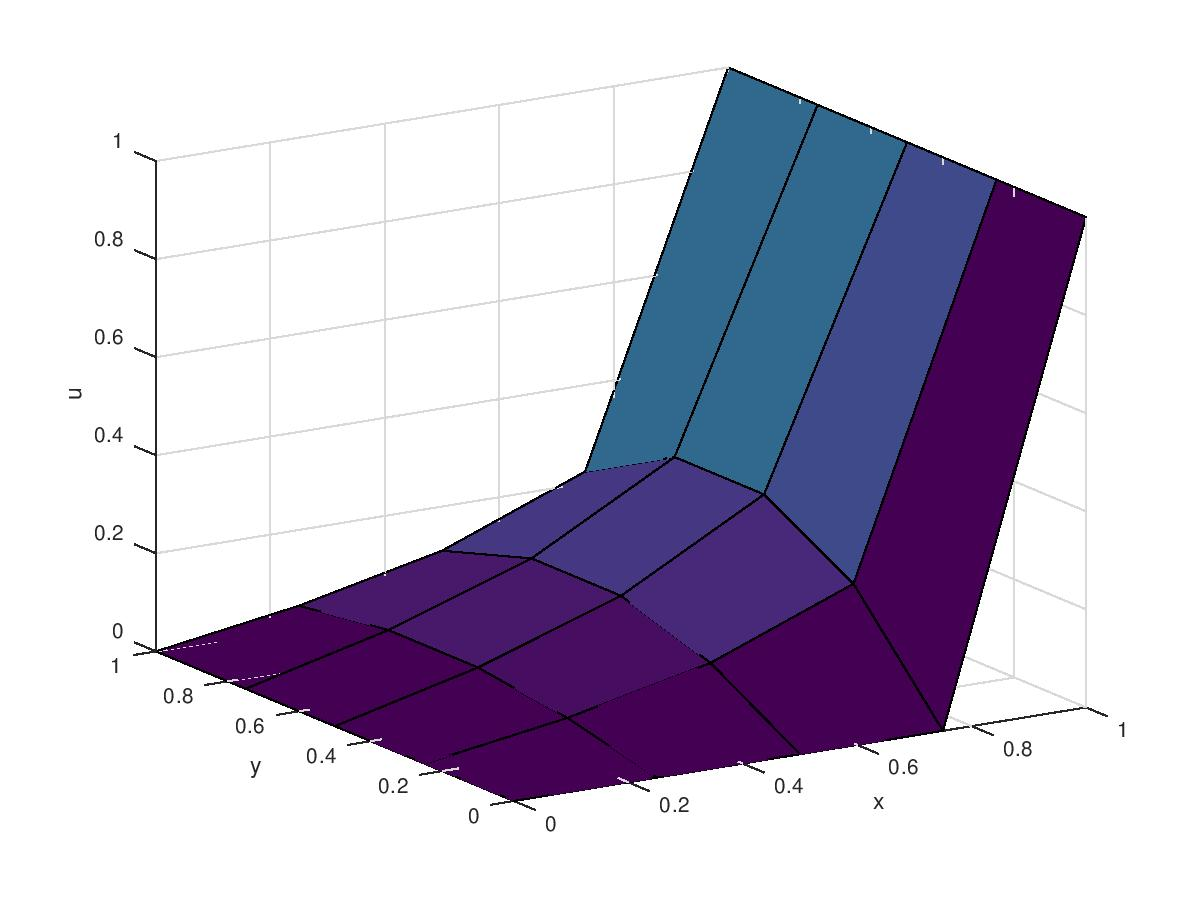
\includegraphics[width=350pt]{w4_1.jpg}

\newpage

\section*{2.}



\end{document}
